\documentclass[aspectratio = 169]{beamer}

\usepackage{slides_tfg}

\begin{document}
	
	% PORTADA
	\begin{frame}[plain]
		\maketitle
	\end{frame}
	
	% ÍNDICE
	\begin{frame}{Índice general}
		\tableofcontents[hideallsubsections]
	\end{frame}
	
	% CONTENIDO
	\section{Introducción}
	
		\subsection{Niantic Wayfarer}
	
			\begin{frame}{Introducción}{Niantic Wayfarer}
				\begin{figure}
					\centering
					\includegraphics[scale = .3]{wayfarer}
				\end{figure}
				\vspace{-.4cm}
				\begin{columns}
					\begin{column}{.3\textwidth}
						\begin{figure}
							\centering
							\includegraphics[height = .5\textheight]{imagen_principal}
						\end{figure}
					\end{column}
					\begin{column}{.3\textwidth}
						\begin{figure}
							\centering
							\includegraphics[height = .45\textheight]{info_principal}
						\end{figure}
					\end{column}
					\begin{column}{.3\textwidth}
						\begin{figure}
							\centering
							\includegraphics[height = .4\textheight]{mapa}
						\end{figure}
					\end{column}
				\end{columns}
			\end{frame}
			
		\subsection{Objetivos}
		
			\begin{frame}{Introducción}{Objetivos}
				\begin{block}{}
					\begin{itemize}
						\item \textbf{Clasificación} de una \textbf{imagen} en un \textbf{conjunto cerrado} de clases
						\item \textbf{Clasificación} de una \textbf{imagen} en un \textbf{conjunto abierto} de clases
						\item \textbf{Búsqueda} de imágenes mediante una descripción \textbf{textual}
						\item Selección del \textbf{título} o \textbf{descripción} más adecuado para una \textbf{imagen}
						\item Aproximación a la detección de \textbf{imágenes} que contienen un \textbf{mismo objeto}
					\end{itemize}
				\end{block}
			\end{frame}
	
	\section{Redes neuronales convolucionales}
	
		\subsection{Proceso ETL}
	
			\begin{frame}{Proceso ETL}{Carga y transformación}
				\begin{columns}
					\begin{column}{.5\textwidth}
						\begin{block}{Algunos problemas...}
							\begin{itemize}
								\item No existe API
								\item Extracción y etiquetado manual
								\item Pocos datos
								\item Clases desbalanceadas
							\end{itemize}
						\end{block}
					\end{column}
					\begin{column}{.5\textwidth}
						\begin{figure}
							\centering
							\includegraphics[width = .9\textwidth]{sample_dataset}
							%\caption{Visualización de ejemplo de un dataset creado}
							\label{fig:sample_dataset}
						\end{figure}
					\end{column}
				\end{columns}
			\end{frame}
			
		\subsection{Red convolucional desde cero}
		
			\begin{frame}{Red neuronal convolucional}{Arquitectura}
				\begin{figure}
					\centering
					\includegraphics[height = .9\textheight]{arq_cnn}
					%\caption{Arquitectura de la red convolucional}
					\label{fig:arq_cnn}
				\end{figure}
			\end{frame}
			\begin{frame}{Tecnologías}{Python y CUDA}
				\begin{columns}
					\begin{column}{.5\textwidth}
						\begin{figure}
							\centering
							\includegraphics[width = .3\textheight, valign = c]{../svg-inkscape/python_svg-raw}\hfill
							\includegraphics[width = .3\textheight, valign = c]{../svg-inkscape/tf_svg-raw}\hfill
							\includegraphics[width = .3\textheight, valign = c]{../svg-inkscape/nvidia_svg-raw}\hfill
						\end{figure}
					\end{column}
					\begin{column}{.5\textwidth}
						\begin{figure}
							\centering
							\includegraphics[height = .75\textheight]{comp_cuda}
%							\caption{Comparativa de entrenamiento en CPU frente a en GPU}
							\label{fig:comparativa_cuda}
						\end{figure}
					\end{column}
				\end{columns}
			\end{frame}
			\begin{frame}{Entrenamiento}{Valores de la función de pérdida}
				\begin{columns}
					\begin{column}{.7\textwidth}
						\begin{block}{}
							\begin{figure}
								\centering
								\includesvg[height = .7\textheight]{epoch_loss_cnn}
								%\caption{Pérdida sobre el conjunto de entrenamiento y validación}
								\label{fig:tb_cnn_c}
							\end{figure}
						\end{block}
					\end{column}
				\end{columns}
			\end{frame}
			
		\subsection{Algunas soluciones al sobreajuste}
		
			\begin{frame}{Medidas contra el sobreajuste}{Aumento de datos}
				\begin{figure}
					\centering
					\includegraphics[height = .8\textheight]{sample_dataset_au}
					%\caption{Visualización de ejemplo de un dataset aplicando aumento de datos}
					\label{fig:sample_dataset_au}
				\end{figure}
			\end{frame}
			
			\begin{frame}{Medidas contra el sobreajuste}{Transfer learning}
				\begin{block}{Con algunas capas de MobileNet}
					\begin{figure}
						\centering
						\includesvg[width = .45\textwidth]{epoch_loss_mb}
						\includesvg[width = .45\textwidth]{epoch_accuracy_mb}
						%\caption{Pérdida sobre el conjunto de entrenamiento y validación}
						\label{fig:tb_tl_c}
					\end{figure}
				\end{block}
			\end{frame}
			
		\subsection{Evaluación de los resultados}
		
			\begin{frame}{Métricas}{Matriz de confusión}
				\begin{figure}
					\centering
					\begin{subfigure}{.4\textwidth}
						\centering
						\includegraphics[height = .7\textheight]{mc_conv}
						\caption{Normal}
						\label{fig:mc_conv}
					\end{subfigure}\hfill
					\begin{subfigure}{.4\textwidth}
						\centering
						\includegraphics[height = .7\textheight]{mc_mb}
						\caption{Aplicando transfer learning}
						\label{fig:mc_mb}
					\end{subfigure}
					%\caption{Matrices de confusión}
					\label{fig:mc}
				\end{figure}
			\end{frame}
			\begin{frame}{Métricas}{Matriz de confusión}
				\begin{figure}
					\centering
					\begin{subfigure}{.4\textwidth}
						\addtocounter{subfigure}{2}
						\centering
						\includegraphics[height = .7\textheight]{mc_convau}
						\caption{Aplicando aumento de datos}
						\label{fig:mc_convau}
					\end{subfigure}\hfill
					\begin{subfigure}{.4\textwidth}
						\centering
						\includegraphics[height = .7\textheight]{mc_mbau}
						\caption{Aplicando ambas}
						\label{fig:mc_mbau}
					\end{subfigure}
					%\caption{Matrices de confusión}
					%\label{fig:mc}
				\end{figure}
			\end{frame}
			\begin{frame}{Métricas}{Precisión, recuerdo, y $F_1-$score}
				\begin{columns}
					\begin{column}{.6\textwidth}
						\begin{block}{}
							\begin{itemize}
								\item Original
								\begin{itemize}
									\item $\mathcal{P} = 0.75$
									\item $\mathcal{R} = 0.743$
									\item $F_1 = 0.728$
								\end{itemize}
								\item Aumento de datos
								\begin{itemize}
									\item $\mathcal{P} = 0.473$
									\item $\mathcal{R} = 0.539$
									\item $F_1 = 0.439$
								\end{itemize}
								\item Transfer learning
								\begin{itemize}
									\item $\mathcal{P} = 0.967$
									\item $\mathcal{R} = 0.967$
									\item $F_1 = 0.967$
								\end{itemize}
							\end{itemize}
						\end{block}
					\end{column}
					\begin{column}{.4\textwidth}
						$$
						\begin{gathered}
							\mathcal{P} = P(C_i | \hat{C}_i)\\
							\mathcal{R} = P(\hat{C}_i | C_i)\\
							F_1 = \frac{2}{\mathcal{P}^{-1} + \mathcal{R}^{-1}}
						\end{gathered}
						$$
					\end{column}
				\end{columns}
			\end{frame}
			\begin{frame}{Métricas}{ROC (OvR) y AUC}
				\begin{figure}
					\centering
					\begin{subfigure}{.4\textwidth}
						\centering
						\includegraphics[height = .7\textheight]{auc_conv}
						\caption{Normal}
						\label{fig:roc_conv}
					\end{subfigure}\hfill
					\begin{subfigure}{.4\textwidth}
						\centering
						\includegraphics[height = .7\textheight]{auc_mb}
						\caption{Aplicando transfer learning}
						\label{fig:roc_mb}
					\end{subfigure}
%					\caption{Curvas ROC}
					\label{fig:roc}
				\end{figure}
			\end{frame}
			\begin{frame}{Métricas}{ROC (OvR) y AUC}
				\begin{figure}
					\centering
					\begin{subfigure}{.4\textwidth}
						\addtocounter{subfigure}{2}
						\centering
						\includegraphics[height = .7\textheight]{auc_convau}
						\caption{Aplicando aumento de datos}
						\label{fig:roc_convau}
					\end{subfigure}\hfill
					\begin{subfigure}{.4\textwidth}
						\centering
						\includegraphics[height = .7\textheight]{auc_mbau}
						\caption{Aplicando ambas}
						\label{fig:roc_mbau}
					\end{subfigure}
%					\caption{Curvas ROC}
%					\label{fig:roc}
				\end{figure}
			\end{frame}
			\begin{frame}{Capacidad de generalización}
				\begin{figure}[!h]
					\centering
					\includegraphics[scale = .65]{gu_vs_ga}
					%\caption{Capacidad de generalización de la red, predicción en Galicia y Guadalajara}
					\label{fig:comparativa_gu}
				\end{figure}
			\end{frame}
			
		\subsection{Conjunto abierto de clases}
		
			\begin{frame}{Conjunto abierto de clases}{Clase \texttt{resto}}
				\begin{columns}
					\begin{column}{.4\textwidth}
						\includegraphics[height = .7\textheight]{mc_open_otros}
					\end{column}
					\begin{column}{.2\textwidth}
						\begin{block}{}
							\begin{itemize}
								\item $\mathcal{P} = 0.958$
								\item $\mathcal{R} = 0.956$
								\item $F_1 = 0.956$
							\end{itemize}
						\end{block}
					\end{column}
					\begin{column}{.4\textwidth}
						\includegraphics[height = .7\textheight]{auc_open_otros}
					\end{column}
				\end{columns}
			\end{frame}
			\begin{frame}[fragile]{Conjunto abierto de clases}{Red neuronal convolucional doble}
				\vspace{-.5cm}
				\begin{columns}
					\begin{column}{.5\textwidth}
						\begin{figure}
							\hspace{-2.5cm}
							\includegraphics[height = .6\textheight]{diagrama_open} 
%							\caption{Arquitectura de clasificación con clases desconocidas}
							\label{fig:openset}
						\end{figure}
					\end{column}
					\begin{column}{.5\textwidth}
						\begin{figure}
							\centering
							$$
							\begin{tikzcd}[ampersand replacement=\&]
								\&  \& R                                                                                      \&  \&        \\
								\texttt{imagen} \arrow[rru, "P(R)", no head] \arrow[rrd, "P(\lnot R)"', no head] \&  \&                                                                                        \&  \& C_1    \\
								\&  \& \lnot R \arrow[rru, "P(C_1|\lnot R)", no head] \arrow[rrd, "P(C_n|\lnot R)"', no head] \&  \& \vdots \\
								\&  \&                                                                                        \&  \& C_n \\
							\end{tikzcd}
							$$
							%\caption{Diagrama de probabilidades}
							\label{fig:prob}
						\end{figure}
					\end{column}
				\end{columns}
			\end{frame}
			\begin{frame}{Conjunto abierto de clases}{Red neuronal convolucional doble}
				\begin{columns}
					\begin{column}{.4\textwidth}
						\includegraphics[height = .7\textheight]{mc_open_bin_multiple}
					\end{column}
					\begin{column}{.22\textwidth}
						\begin{block}{}
							\begin{itemize}
								\item $\mathcal{P} = 0.945$
								\item $\mathcal{R} = 0.945$
								\item $F_1 = 0.945$
							\end{itemize}
						\end{block}
					\end{column}
					\begin{column}{.4\textwidth}
						\includegraphics[height = .7\textheight]{auc_open_bin_multiple}
					\end{column}
				\end{columns}
			\end{frame}
	
	\section{Transformers multimodales}
	
		\subsection{Generación de embeddings multimodales}
	
			\begin{frame}{Transformers multimodales}{Embeddings multimodales}
				\begin{columns}
					\begin{column}{.5\textwidth}
						\begin{block}{}
							\begin{figure}
								\centering
								\includegraphics[height = .7\textheight]{diagrama_embeddings}
								%					\caption{Concepto de embeddings de un transformer multimodal}
								\label{fig:diagrama_embeddings}
							\end{figure}
						\end{block}
					\end{column}
				\end{columns}
			\end{frame}
	
		
			\begin{frame}{Generación de embeddings multimodales en VertexAI}
				\centering\resizebox{\textwidth}{!}{
					\tikzset{every picture/.style={line width=0.75pt}} %set default line width to 0.75pt    
					\begin{tikzpicture}[x=0.75pt,y=0.75pt,yscale=-1,xscale=1]
						%uncomment if require: \path (0,300); %set diagram left start at 0, and has height of 300
						
						%Image [id:dp49735390400769464] 
						\draw (579.7,144.8) node  {\includegraphics[width=52.5pt,height=52.5pt]{gcp.png}};
						%Straight Lines [id:da8970164609460181] 
						\draw    (199.3,70.6) -- (305.5,70.6) ;
						\draw [shift={(308.5,70.6)}, rotate = 180] [fill={rgb, 255:red, 0; green, 0; blue, 0 }  ][line width=0.08]  [draw opacity=0] (8.93,-4.29) -- (0,0) -- (8.93,4.29) -- cycle    ;
						%Straight Lines [id:da33929728234036016] 
						\draw    (197.7,221.4) -- (304.3,221.4) ;
						\draw [shift={(307.3,221.4)}, rotate = 180] [fill={rgb, 255:red, 0; green, 0; blue, 0 }  ][line width=0.08]  [draw opacity=0] (8.93,-4.29) -- (0,0) -- (8.93,4.29) -- cycle    ;
						%Rounded Rect [id:dp4478793620612258] 
						\draw  [fill={rgb, 255:red, 255; green, 255; blue, 255 }  ,fill opacity=1 ] (316.9,59) .. controls (316.9,43.32) and (329.62,30.6) .. (345.3,30.6) -- (430.5,30.6) .. controls (446.18,30.6) and (458.9,43.32) .. (458.9,59) -- (458.9,230.6) .. controls (458.9,246.28) and (446.18,259) .. (430.5,259) -- (345.3,259) .. controls (329.62,259) and (316.9,246.28) .. (316.9,230.6) -- cycle ;
						%Straight Lines [id:da30336065089279907] 
						\draw    (471.5,149.8) -- (533.9,149.8) ;
						\draw [shift={(536.9,149.8)}, rotate = 180] [fill={rgb, 255:red, 0; green, 0; blue, 0 }  ][line width=0.08]  [draw opacity=0] (8.93,-4.29) -- (0,0) -- (8.93,4.29) -- cycle    ;
						\draw [shift={(468.5,149.8)}, rotate = 0] [fill={rgb, 255:red, 0; green, 0; blue, 0 }  ][line width=0.08]  [draw opacity=0] (8.93,-4.29) -- (0,0) -- (8.93,4.29) -- cycle    ;
						%Straight Lines [id:da1644899983955368] 
						\draw    (201.9,101) -- (308.1,101) ;
						\draw [shift={(198.9,101)}, rotate = 0] [fill={rgb, 255:red, 0; green, 0; blue, 0 }  ][line width=0.08]  [draw opacity=0] (8.93,-4.29) -- (0,0) -- (8.93,4.29) -- cycle    ;
						%Straight Lines [id:da1968388191399162] 
						\draw    (200.7,191) -- (306.9,191) ;
						\draw [shift={(197.7,191)}, rotate = 0] [fill={rgb, 255:red, 0; green, 0; blue, 0 }  ][line width=0.08]  [draw opacity=0] (8.93,-4.29) -- (0,0) -- (8.93,4.29) -- cycle    ;
						
						% Text Node
						\draw (146.7,61) node [anchor=north west][inner sep=0.75pt]   [align=left] {{Imagen}};
						% Text Node
						\draw (149.5,209.8) node [anchor=north west][inner sep=0.75pt]   [align=left] {{Texto}};
						% Text Node
						\draw (363.5,112.2) node [anchor=north west][inner sep=0.75pt]   [align=left] {\begin{minipage}[lt]{39.12pt}\setlength\topsep{0pt}
								\begin{center}
									{{\Large API}}\\{{\Large REST}}
								\end{center}
								
						\end{minipage}};
						% Text Node
						\draw (11.4,91.1) node [anchor=north west][inner sep=0.75pt]   [align=left] {{Embedding imagen}};
						% Text Node
						\draw (19.9,181.9) node [anchor=north west][inner sep=0.75pt]   [align=left] {{Embedding texto}};
						% Text Node
						\draw (131,89.4) node [anchor=north west][inner sep=0.75pt]    {$\in\mathbb{R}^{1408}$};
						% Text Node
						\draw (127.5,180.4) node [anchor=north west][inner sep=0.75pt]    {$\in\mathbb{R}^{1408}$};
					\end{tikzpicture}
				}
			\end{frame}
			
			\begin{frame}{Embeddings en $\mathbb{R}^2$}{PCA y t-SNE}
				\begin{block}{}
					\begin{figure}
						\centering
						\includegraphics[width = \textwidth]{reduced_embeddings}
						%					\caption{Embeddings en $\mathbb{R}^2$ mediante PCA y t-SNE}
						\label{fig:embeddingsR2}
					\end{figure}
				\end{block}
			\end{frame}
			
		\subsection{Clasificación no supervisada}
		
			\begin{frame}{Clasificación no supervisada}{$k-$means}
				\begin{block}{}
					\begin{figure}
						\centering
						\includegraphics[width = \textwidth]{reduced_embeddings_k-means}
%						\caption{Clusters calculados con $k-$means}
						\label{fig:clusters_kmeans}
					\end{figure}
				\end{block}
			\end{frame}
			\begin{frame}{Clasificación no supervisada}{Clustering jerárquico aglomerativo}
				\begin{block}{}
					\begin{figure}
						\centering
						\includegraphics[width = \textwidth]{reduced_embeddings_Clustering jerárquico aglomerativo}
%						\caption{Clusters calculados con CJA}
						\label{fig:clusters_cja}
					\end{figure}
				\end{block}
			\end{frame}
			\begin{frame}{Clasificación no supervisada}
				\vspace{-2cm}
				\hspace{1.5cm}
				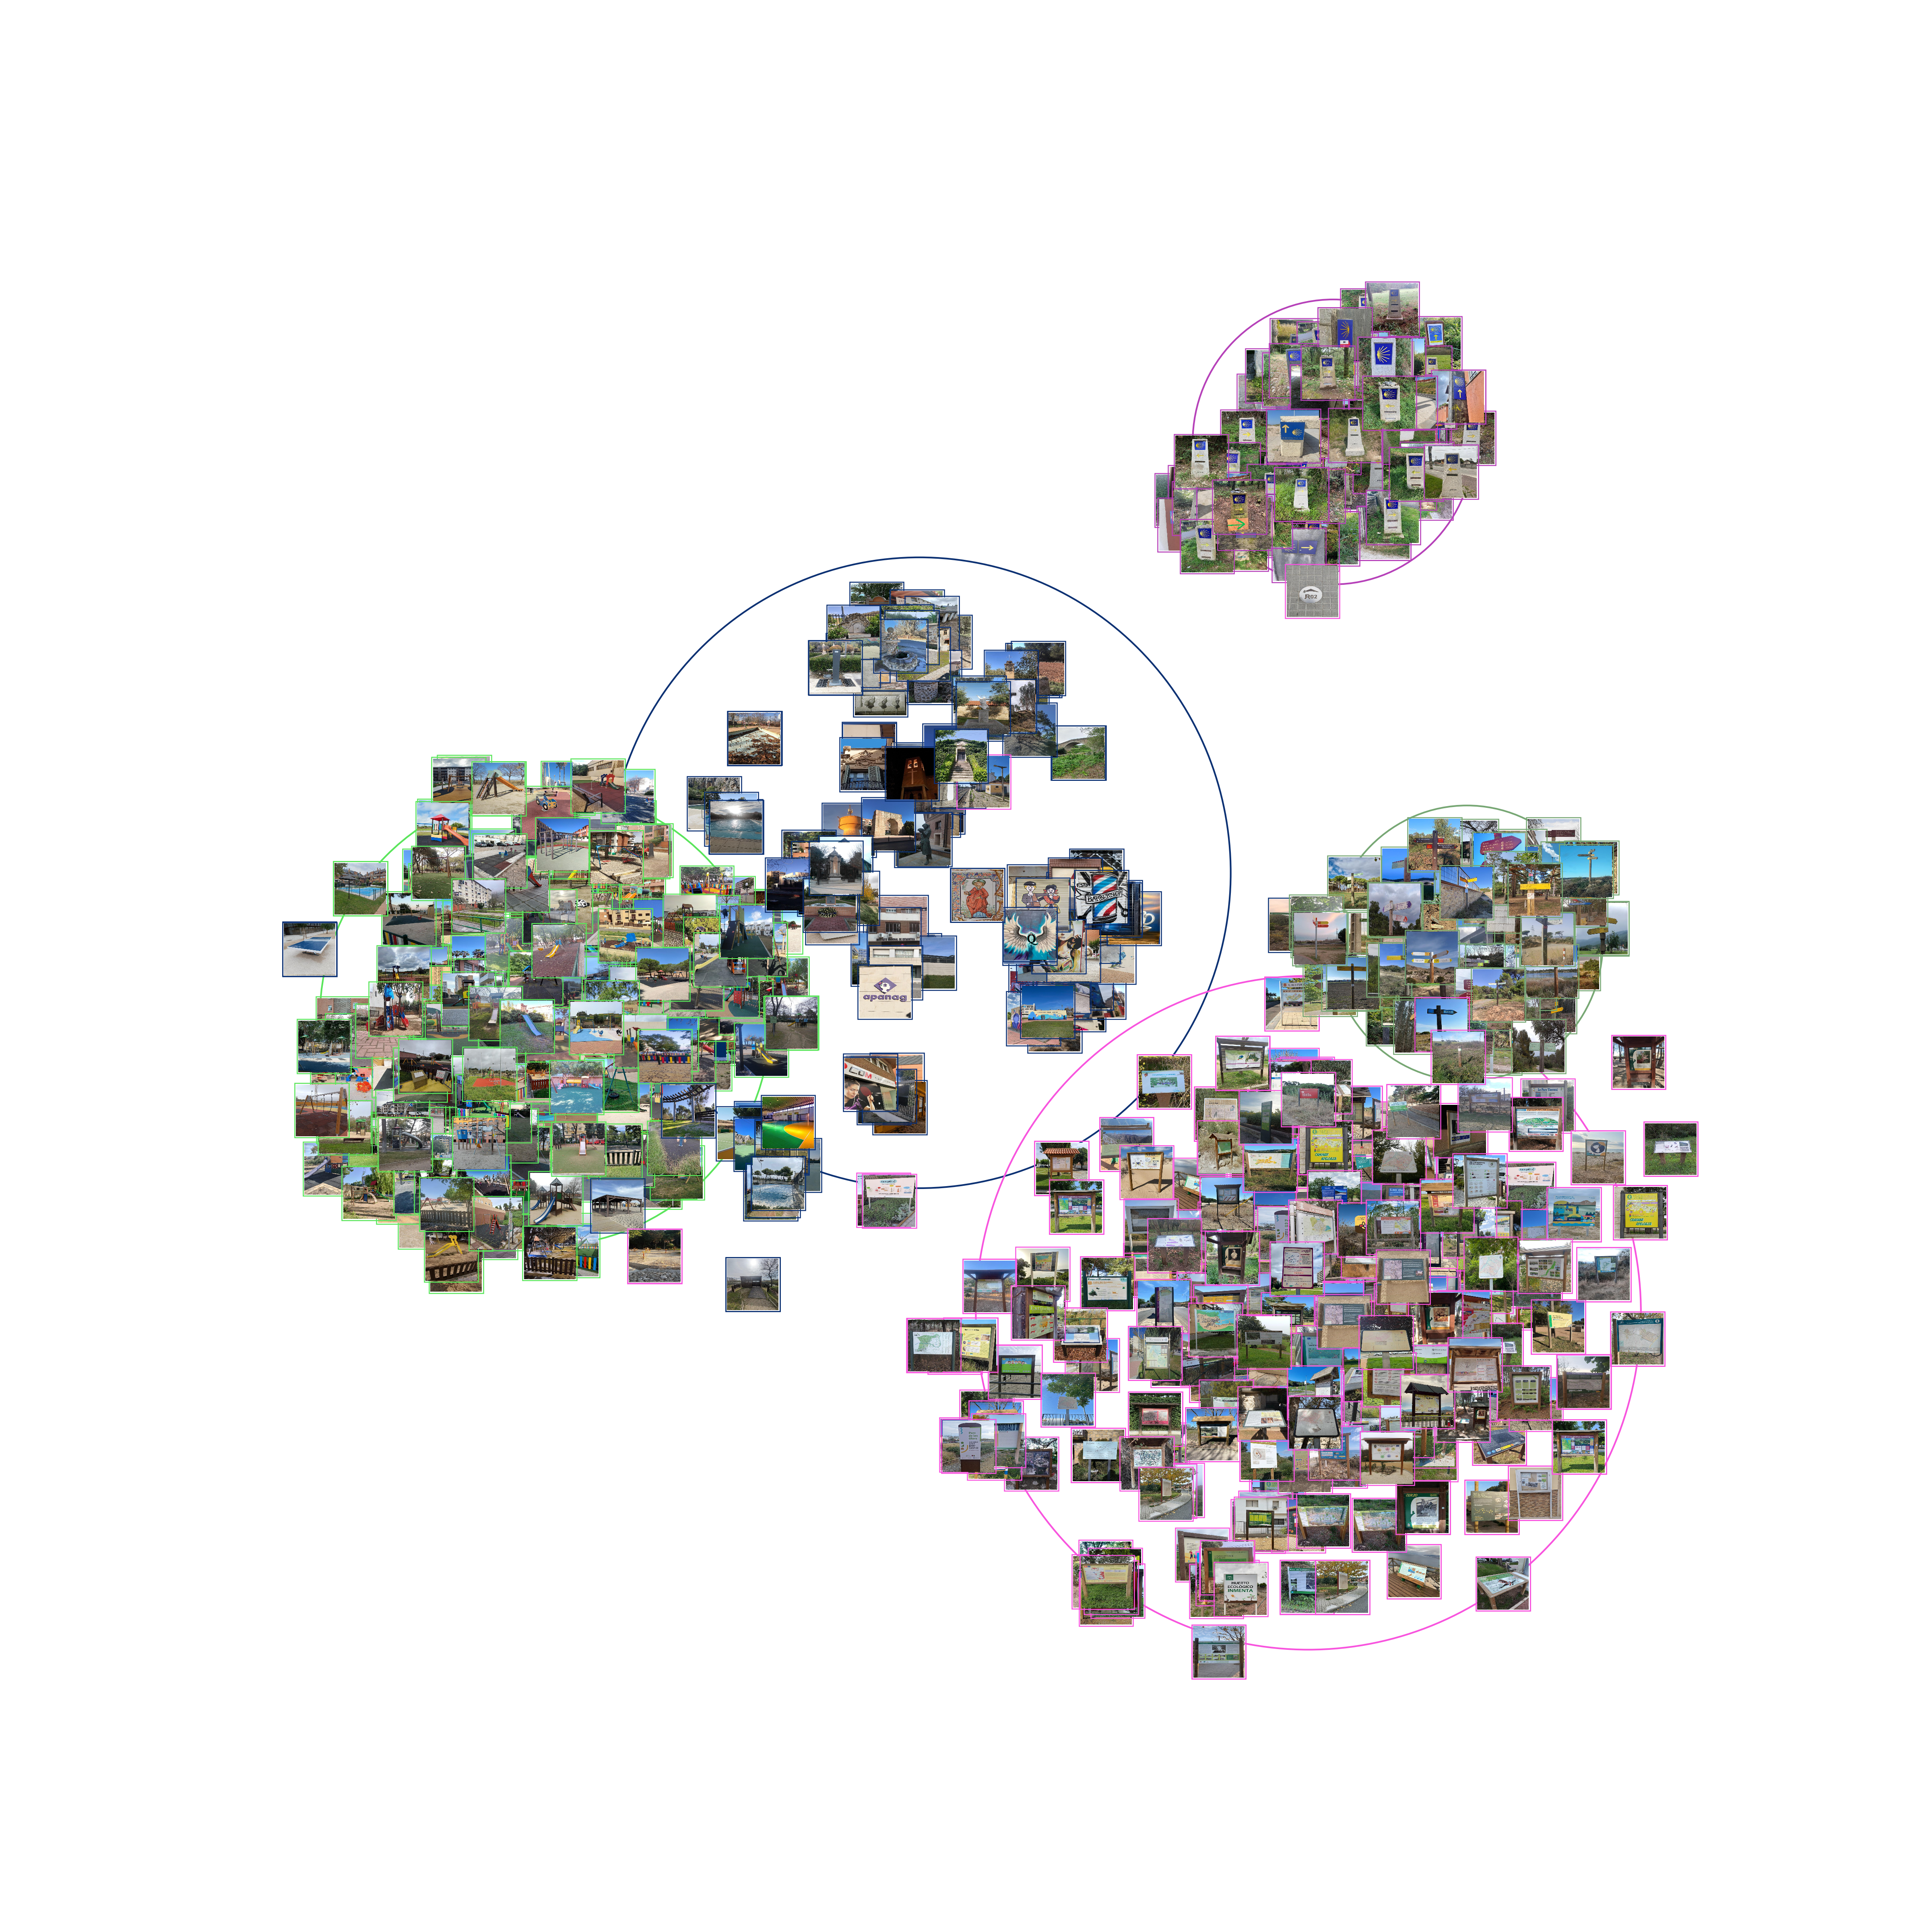
\includegraphics[scale = .05]{images_clusters}
			\end{frame}
			\begin{frame}{¿Y si no se conoce el número de clusters?}{Método del codo y kneedle}
				\begin{figure}
					\centering
					\includegraphics[height = .8\textheight]{elbow_kmeans}
					%						\caption{Cálculo del $k$ óptimo mediante el método del codo}
					\label{fig:elbow}
				\end{figure} 
			\end{frame}
		
		\subsection{Métricas}
		
			\begin{frame}{Métricas}{Coeficiente de la silueta}
				\begin{figure}
					\centering
					\includegraphics[height = .8\textheight]{silhouette_kmeans}
%					\caption{Coeficiente de la silueta para $k-$means}
					\label{fig:silhouette_kmeans}
				\end{figure} 
			\end{frame}
			
			\begin{frame}{Métricas}{Matrices de contingencia}
				\begin{figure}
					\centering
					\includegraphics[width = \textwidth]{matrices_contingencia}
%					\caption{Matrices de contingencia}
					\label{fig:matrices_contingencia}
				\end{figure} 
			\end{frame}
			
			\begin{frame}{Métricas}{Matrices de confusión}
				\begin{figure}
					\centering
					\includegraphics[width = \textwidth]{matrices_confusion_transf}
%					\caption{Matrices de confusión}
					\label{fig:matrices_confusion_transf}
				\end{figure} 
			\end{frame}
			
			\begin{frame}{Métricas}{ARI y $V-$measure}
				\begin{columns}
					\begin{column}{.5\textwidth}
						\begin{block}{$k-$means}
							\begin{itemize}
								\item ARI: $0.944$
								\item $V-$measure: $0.932$
							\end{itemize}
						\end{block}
					\end{column}
					\begin{column}{.5\textwidth}
						\begin{block}{CJA}
							\begin{itemize}
								\item ARI: $0.953$
								\item $V-$measure: $0.938$
							\end{itemize}
						\end{block}
					\end{column}
				\end{columns}
				\vfill\centering Cuidado si hay pocas observaciones y/o muchos clusters...
			\end{frame}
			
		\subsection{Asignación de textos}
		
			\begin{frame}{Búsqueda semántica de imágenes}
				\begin{block}{}
					Encontrar las imágenes que mejor se ajustan a una descripción textual
					$$
					-1\leq\cos(\theta)\leq 1
					$$
					\begin{itemize}
						\item Parque infantil
						\item Marcador de ruta
						\item Cartel informativo
						\item Fuentes, piscinas, y elementos de agua
						\item Murales, grafitis, dibujos, y arte
					\end{itemize}
				\end{block}
			\end{frame}
			\begin{frame}{Búsqueda semántica de imágenes}
				\begin{figure}
					\centering
					\includegraphics[height = .8\textheight]{busqueda_parque}
				\end{figure} 
			\end{frame}
			\begin{frame}{Búsqueda semántica de imágenes}
				\begin{figure}
					\centering
					\includegraphics[height = .8\textheight]{busqueda_marcadores}
				\end{figure} 
			\end{frame}
			\begin{frame}{Búsqueda semántica de imágenes}
				\begin{figure}
					\centering
					\includegraphics[height = .8\textheight]{busqueda_carteles}
				\end{figure} 
			\end{frame}
			\begin{frame}{Búsqueda semántica de imágenes}
				\begin{figure}
					\centering
					\includegraphics[height = .8\textheight]{busqueda_arte}
				\end{figure} 
			\end{frame}
			\begin{frame}{Búsqueda semántica de imágenes}
				\begin{figure}
					\centering
					\includegraphics[height = .8\textheight]{busqueda_agua}
				\end{figure} 
			\end{frame}
			\begin{frame}{Búsqueda semántica de imágenes}
				\begin{figure}
					\centering
					\includegraphics[height = .8\textheight]{cartel_busqueda}
				\end{figure} 
			\end{frame}	
	
	\section{Conclusiones y trabajo futuro}
		
		\subsection{Objetivos logrados}
	
			\begin{frame}{Conclusiones y trabajo futuro}
				\begin{block}{Logros}
					\begin{itemize}
						\item \textbf{Clasificación} de imágenes en \textbf{conjuntos abiertos} y \textbf{cerrados}, de manera \textbf{supervisada} y \textbf{no supervisada}
						\item \textbf{Selección} de \textbf{textos descriptivos} para las imágenes 
					\end{itemize}
				\end{block}
			\end{frame}
			
		\subsection{Trabajo futuro}
		
			\begin{frame}{Conclusiones y trabajo futuro}
				\begin{block}{Para automatizar al completo el proceso...}
					\begin{itemize}
						\item Verificación de coordenadas
						\item Detección de elementos duplicados
					\end{itemize}
				\end{block}
				\begin{figure}
					\centering
					\includegraphics[width = .85\textwidth]{duplicados}
	%				\caption{Imágenes entre las que detectar duplicados}
					\label{fig:duplicados}
				\end{figure}
				$$
				0.89 \qquad 0.75 \qquad 0.44 \qquad 0.49
				$$
			\end{frame}
	
	% PORTADA CIERRE
	\begin{frame}[plain]
		\maketitle
	\end{frame}
\end{document}